\documentclass{article}
\usepackage{tikz}
\usetikzlibrary{automata,positioning,arrows.meta}

\begin{document}

\title{CSI 3430: Test One}

\date{}

\maketitle

\section*{Instruction}

This closed book test has 8 pages inclusive and there are 9 questions to answer. Please check if you
have a complete test paper before proceeding to questions.
\vspace{2pc}

 \noindent
Your handwriting must be legible. \vspace{2pc}

\noindent Write your name below. \vspace{2pc}

\noindent {\bf Student name:}


\pagebreak

\section*{Questions}

\begin{enumerate}
\item Let ODD be the set of all odd natural numbers. Give an
  inductive definition for ODD and show a proof tree for $5\in ODD$.

\pagebreak

\item A set of sets $\mathcal{S}$ is called closed under union if the
  union of any two sets in $\mathcal{S}$ is also in $\mathcal{S}$. The
  closure-under-union of a set of sets $\mathcal{T}$, denoted
  $C(\mathcal{T})$, is the smallest $\mathcal{S}$ such that
  $\mathcal{T}\subseteq\mathcal{S}$ and $\mathcal{S}$ is closed under
  union.  Give an inductive definition for $C(\mathcal{T})$.

\pagebreak

%\item Prove by induction that $\Sigma_{i=1}^n i = \frac{n(n+1)}{2}$.
%\vspace{15pc}

\item Let $L=\{ab,aa,a\}$. Argue that $aaabaa$ is in $L^*$.
\vspace{15pc}


\item Let $\Sigma=\{a,b\}$ be the alphabet. Write a regular
expression that generates all strings of a's and b's except those
that contain ab as a substring. \pagebreak


\item Let $\Sigma=\{a,b,c\}$ be the alphabet. Write a regular
expression that generates all those strings over $\Sigma$ in which
all letters in $\Sigma$ occur in doubles.

\vspace{10pc}

\item Write a regular expression that generates $L((a+b)^*) -
L((a+b)^*a(a+b)^*)$. \vspace{10pc}

\item Construct a finite automaton that accepts all those strings
over $\Sigma=\{a,b\}$ that contain aab as a substring.

\pagebreak

 \item Let M be the  finite automaton depicted below. Give a concise description of the language
 accepted by M in English.

\begin{center}
\resizebox{.5\textwidth}{!}{%
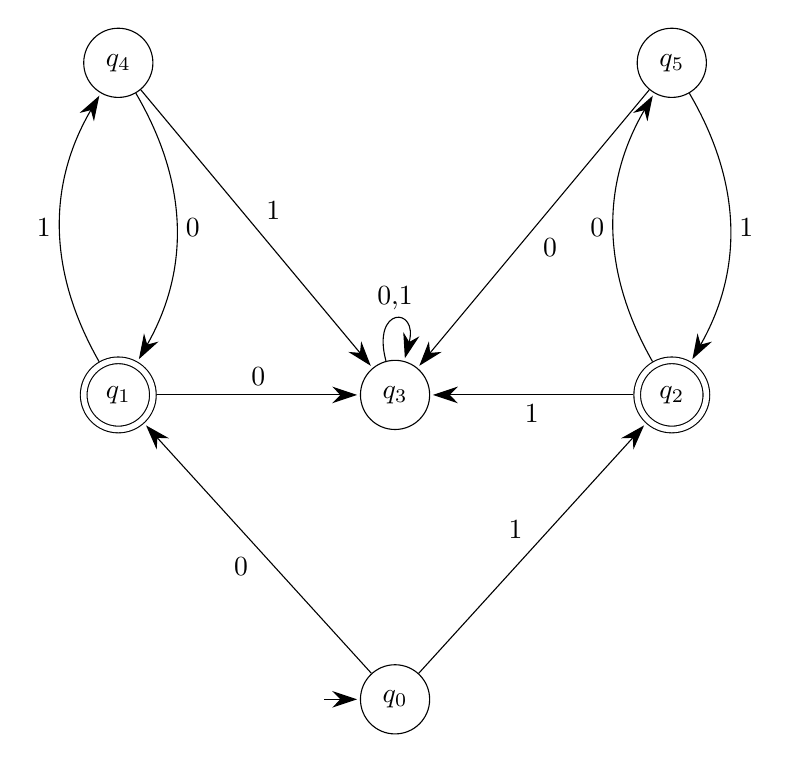
\begin{tikzpicture}[>={Stealth[width=6pt,length=9pt]}, accepting/.style={double distance = 2pt, outer sep = 1pt + \pgflinewidth}, shorten >=1pt, auto]
  \draw (120.0pt, -280.0pt)node[state, initial, initial text =](0){$q_{0}$};
  \draw (20.0pt, -170.0pt)node[state, accepting](1){$q_{1}$};
  \draw (220.0pt, -170.0pt)node[state, accepting](2){$q_{2}$};
  \draw (120.0pt, -170.0pt)node[state](3){$q_{3}$};
  \draw (20.0pt, -50.0pt)node[state](4){$q_{4}$};
  \draw (220.0pt, -50.0pt)node[state](5){$q_{5}$};
  \path[->] (5) edge[bend left] node{1}(2);
  \path[->] (2) edge node{1}(3);
  \path[->] (2) edge[bend left] node{0}(5);
  \path[->] (5) edge node{0}(3);
  \path[->] (0) edge node{1}(2);
  \path[->] (4) edge node{1}(3);
  \path[->] (3) edge[loop above] node{0,1}(3);
  \path[->] (1) edge node{0}(3);
  \path[->] (1) edge[bend left] node{1}(4);
  \path[->] (0) edge node{0}(1);
  \path[->] (4) edge[bend left] node{0}(1);
\end{tikzpicture}
}%
\end{center}

\pagebreak

\item Obtain a regular expression that generates the language
accepted by the finite automaton depicted below. You need to draw the Generalized Transition Graph obtained after each step. Elimination of
a state is considered as one step.

\begin{center}
\resizebox{.3\textwidth}{!}{%
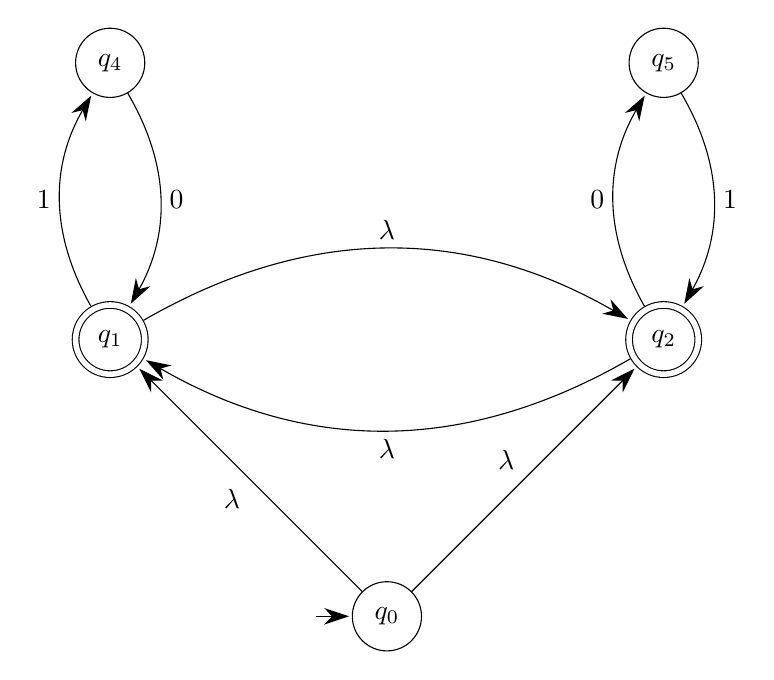
\begin{tikzpicture}[>={Stealth[width=6pt,length=9pt]}, accepting/.style={double distance = 2pt, outer sep = 1pt + \pgflinewidth}, shorten >=1pt, auto]
  \draw (120.0pt, -250.0pt)node[state, initial, initial text =](0){$q_{0}$};
  \draw (20.0pt, -150.0pt)node[state, accepting](1){$q_{1}$};
  \draw (220.0pt, -150.0pt)node[state, accepting](2){$q_{2}$};
  \draw (20.0pt, -50.0pt)node[state](4){$q_{4}$};
  \draw (220.0pt, -50.0pt)node[state](5){$q_{5}$};
  \path[->] (5) edge[bend left] node{1}(2);
  \path[->] (2) edge[bend left] node{0}(5);
  \path[->] (0) edge node{$\lambda$}(2);
  \path[->] (1) edge[bend left] node{$\lambda$}(2);
  \path[->] (2) edge[bend left] node{$\lambda$}(1);
  \path[->] (1) edge[bend left] node{1}(4);
  \path[->] (4) edge[bend left] node{0}(1);
  \path[->] (0) edge node{$\lambda$}(1);
\end{tikzpicture}
}%
\end{center}

\pagebreak

\mbox{}
\end{enumerate}
\end{document}

\pagebreak

%\item 
Let $M_1$ and $M_2$ be the finite automata depicted below ($M_1$
  is depicted above $M_2$). Construct a finite automaton $M$ such that
  $L(M)=L(M_1)\cap L(M_2)$ using a systematic approach where $\cap$ is
  set intersection. Show steps please.

\begin{center}
\resizebox{.5\textwidth}{!}{%
\begin{tikzpicture}[>={Stealth[width=6pt,length=9pt]}, accepting/.style={double distance = 2pt, outer sep = 1pt + \pgflinewidth}, shorten >=1pt, auto]
  \draw (200.0pt, -50.0pt)node[state](0){$s_{3}$};
  \draw (50.0pt, -150.0pt)node[state, initial, initial text ={$M_1$}](1){$s_{0}$};
  \draw (200.0pt, -150.0pt)node[state](2){$s_{1}$};
  \draw (350.0pt, -150.0pt)node[state, accepting](3){$s_{2}$};

  \draw (50.0pt, -300.0pt)node[state, initial, initial text ={$M_2$}, accepting](4){$t_{0}$};
  \draw (350.0pt, -300.0pt)node[state](5){$t_{1}$};
  \path[->] (3) edge [bend right] node[above]{0}(0);
  \path[->] (4) edge[loop above] node{0}(4);
  \path[->] (5) edge[loop above] node{0}(5);
  \path[->] (0) edge[loop above] node{0,1}(0);
  \path[->] (2) edge[bend left] node{0}(3);
  \path[->] (3) edge[bend left] node{1}(2);
  \path[->] (2) edge node{1}(0);
  \path[->] (1) edge node{0}(0);
  \path[->] (4) edge[bend left] node{1}(5);
  \path[->] (5) edge[bend left] node{1}(4);
  \path[->] (1) edge node{1}(2);
\end{tikzpicture}
}%

\end{center}
\end{document}